\documentclass{article}
\usepackage[utf8]{inputenc}
\usepackage{enumitem}
\usepackage{graphicx}

\title{Reeksamen 2015}
\author{kiettn12, Jeppe Bartel (jebar20)}
\date{\today}

\begin{document}

\maketitle

\section{Reeksamen februar 2015 opgave 3}
Lad R, S og T være relationer på mængden {1, 2, 3, 4}.\\

a) 
Lad R =  {(1, 1),(2, 1),(2, 2),(2, 4),(3, 1),(3, 3),(3, 4),(4, 1),(4, 4)}.\\
Er R en partiel ordning?\\
Ja. Da relationen er refleksiv (alle noder har en loop til sig selv), antisymmetrisk (der er ingen kanter, der går i begge retninger) og transitiv.\\

b) Lad S = {(1, 2),(2, 3),(2, 4),(4, 2)}. 
Angiv den transitive lukning af S.\newline
$S^1$ = {(1, 2),(2, 3),(2, 4),(4, 2)}\newline
$S^2$ = {(1, 3), (1, 4), (2, 2), (4, 3), (4, 4)}\\
$S^*$ = $S^1$ \cup $S^2$\\
$S^*$ = {(1, 2), (1, 3), (1, 4), (2, 2),(2, 3),(2, 4),(4, 2), (4, 3), (4, 4)}\\

c) Lad T = {(1, 1),(1, 3),(2, 2),(2, 4),(3, 1),(3, 3),(4, 2),(4, 4)}. Bemærk at T er en ækvivalens-relation.\\
Angiv Ts ækvivalens-klasser:
{(1, 1), (1, 3), (3, 1), (3, 3)}, {(2, 2), (2, 4), (4, 2), (4, 4)}.\\

ekstra) Angiv matricerne for de tre relationer R, S og T.\\
R:\\
\begin{bmatrix}
1 & 1 & 1 & 1\\
0 & 1 & 0 & 0\\
0 & 0 & 1 & 0\\
0 & 1 & 1 & 1\\
\end{bmatrix}
\\
\\
S:\\
\begin{bmatrix}
0 & 0 & 0 & 0\\
1 & 0 & 0 & 1\\
0 & 1 & 0 & 0\\
0 & 1 & 0 & 0\\
\end{bmatrix}
\\
\\
T:\\
\begin{bmatrix}
1 & 0 & 1 & 0\\
0 & 1 & 0 & 1\\
1 & 0 & 1 & 0\\
0 & 1 & 0 & 1\\
\end{bmatrix}

\section{Eksamen januar 2009 opgave 3}
Lad S = {1, 2, . . . , 15}. Betragt følgende binære relation på S\\
R = {(a, b) | b = 2a}\\\\
a) Hvilke af nedenstående par tilhører R? Hvilke tilhører $R^2$?\\
(1, 1), (2, 4), (4, 2), (3, 5), (2, 8)\\
//
(2,4) tilhører R.
(2, 8) tilhører $R^2$.\\\\
b) Opskriv alle par i den transitive lukning af R.\\
R = {(1, 2), (2, 4), (3, 6), (4, 8), (5, 10), (6, 12), (7, 14)}.\\
$R^2$ = {(1, 4), (2, 8), (3, 12)}.\\
$R^3$ = {(1, 8)}\\
$R^*$ = R \cup $R^2$ \cup $R^3$\\
$R^*$ = {(1, 2), (1, 4), (1, 8), (2, 4), (2, 8), (3, 6), (3, 12), 4, 8), (5, 10), (6, 12), (7, 14)}\\

ekstra) Opskriv desuden matricen, der repræsenterer relationen R, dog med S = {1, 2, ..., 6}.\\
\begin{bmatrix}
0 & 0 & 0 & 0 & 0 & 0\\
1 & 0 & 0 & 0 & 0 & 0\\
0 & 0 & 0 & 0 & 0 & 0\\
0 & 1 & 0 & 0 & 0 & 0\\
0 & 0 & 0 & 0 & 0 & 0\\
0 & 0 & 1 & 0 & 0 & 0\\
\end{bmatrix}

\title{
\normalsize \normalfont
\textbf{Opgave 1}}
\\
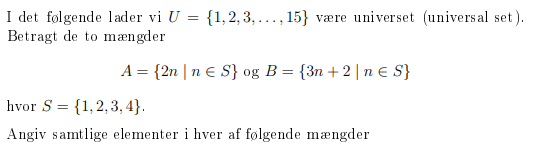
\includegraphics[width=1.0 \textwidth]{Reeksamen.PNG}
\begin{enumerate}[label=(\Alph*)]
\item $A
\\
$A = \big\{2,4,6,8\big\}
\\

\item $B 
\\
$B = \big\{5,8,11,14\big\}
\\

\item $A \cap $B 
\\
$A \cap $B = \big\{8\big\}
\\

\item $A\cup$B 
\\
$A\cup$B = \big\{2,4,5,6,8,11,13\big\}
\\

\item $A-B$
\\
A-B= \big\{2,4,6\big\}
\\

\item \overline{A}
\\ 
\overline{A} = \big\{1,3,5,7,9,10,11,12,13,14,15\big\}
\\

\end{enumerate}
\\



\end{document}
